% IEEE-format article derived from coursework experiments (CS 6343-style seed).
% Section files follow the multi-author layout from:
% https://github.com/mister-weeden/et-al-Masapeta-Dhakal-Ravula-Zhang (CVPR_1494/sec/* pattern).
% Build: pdflatex or latexmk from this directory; requires IEEEtran (e.g. texlive-publishers).
\documentclass[conference]{IEEEtran}
\usepackage{cite}
\usepackage{amsmath,amssymb}
\usepackage{graphicx}
\usepackage{url}
% Peer-review style annotations (aligned with et-al-Masapeta-Dhakal-Ravula-Zhang review_commands_reference.md)
\usepackage[table,dvipsnames]{xcolor}
\newcommand{\strength}[1]{\textcolor{ForestGreen!90!black}{\textbf{Strength:} #1}}
\newcommand{\weakness}[1]{\textcolor{red!75!black}{\textbf{Weakness:} #1}}
\newcommand{\suggestion}[1]{\textcolor{blue!75!black}{\textbf{Suggestion:} #1}}

\usepackage{hyperref}

% Figures from scripts/run_coursework_outputs.py (conda env rd-ralph-template)
\graphicspath{{../output/diagrams/}}

\hypersetup{hidelinks}

\title{Experimental Analysis of AES Diffusion, Block Cipher Modes, and TLS Cipher Suites}

\author{
\IEEEauthorblockN{Author Name}
\IEEEauthorblockA{\textit{Department} \\
\textit{University}\\
email@domain}
}

\begin{document}
\maketitle

\begin{abstract}
We present an empirical study seeded by structured cryptography coursework, extending assignment questions into reproducible experiments suitable for archival reporting. We measure AES round-by-round avalanche behavior under controlled modifications (ShiftRows and MixColumns variants), compare ECB and CBC mode leakage on structured bitmap data, and summarize TLS cipher suite negotiations from a small browser and website sample. We discuss limitations, reproducibility, and relation to standardization practice.
\end{abstract}

\begin{IEEEkeywords}
AES, avalanche effect, block cipher modes, ECB, CBC, TLS, cipher suites, reproducibility
\end{IEEEkeywords}

% --- Body (same \input order as CVPR_1494/main.tex in the reference template) ---
% Section 0 | Executive Summary | Lead: Phaninder Reddy Masapeta
\section{Executive Summary}
\label{sec:executive-summary}

\strength{This manuscript turns structured cryptography coursework into reproducible experiments with clear metrics (Hamming traces, visual mode comparison, TLS negotiation snapshots) and explicit artifact paths.}

We summarize three experiment tracks: (i) AES-128 round-by-round diffusion under plaintext/key perturbations and component ablations; (ii) ECB versus CBC on bitmap data with header-repair visualization; (iii) a finite sample of TLS handshakes and negotiated parameters across hosts.

\weakness{Scope is intentionally course-scale: small TLS samples and educational AES code are not substitutes for production cryptography evaluation.}

\suggestion{Prominently separate ``teaching implementation'' from ``security certification'' in the abstract and executive summary for external readers.}

% Section 1 | Technical Contribution | Akhila Ravula
\section{Technical Contribution}
\label{sec:technical-contribution}

Block ciphers and their modes remain central to real-world security, from disk encryption to TLS~\cite{daemen2002design}. This work uses a homework-driven methodology to ensure concrete, checkable tasks, then reframes results as a journal-style contribution with explicit methodology and threats to validity.

\strength{Contributions are operational: logged AES states with byte/bit Hamming summaries, paired ECB/CBC ciphertext visualizations, and tabular TLS negotiation summaries tied to repository scripts and outputs.}

\suggestion{Add a one-paragraph ``claims'' list (bullet form) mirroring the three assignment questions so reviewers can map sections to obligations quickly.}

% Section 2 | Experimental Methodology | Zezheng Zhang
\section{Experimental Methodology}
\label{sec:experimental-methodology}

\subsection{Question 1: AES tracing and diffusion metrics}
We implement or instrument AES-128 with logged intermediate states after AddRoundKey, SubBytes, ShiftRows, MixColumns (round 10 omits MixColumns). Hamming distances (byte and bit) compare nominal versus single-bit plaintext and key perturbations. Ablations disable ShiftRows or replace the MixColumns matrix as specified in the assignment brief.

\subsection{Question 2: ECB versus CBC on bitmap data}
OpenSSL (or equivalent) encrypts a fixed test image in ECB and CBC with a random 16-byte key and IV. We document visual artifacts, then restore the BMP header from plaintext to observe corrected viewing behavior and interpret mode-dependent structure.

\subsection{Question 3: TLS handshake observation}
Wireshark captures Client Hello and Server Hello cipher suites for multiple browsers and sites. We classify algorithms (key exchange, authentication, bulk cipher/mode, MAC where applicable) and note TLS~1.3 differences from TLS~1.2 decomposition.

\section{Experimental Setup}
\label{sec:experimental-setup}
Experiments are specified under \texttt{test\_cases/} and executed artifacts are written to \texttt{output/results/} and \texttt{output/diagrams/}. Environment versions (OpenSSL, Wireshark, OS) are recorded for reproducibility.

% Section 3 | Results \& Claims Validation | Sriya Dhakal
\section{Results and Claims Validation}
\label{sec:results-validation}

\subsection{Question 1: AES diffusion and ablations}
Figure~\ref{fig:q1-hamming-rounds} traces bit-level Hamming distance between internal states for all-zero plaintext versus a one-bit perturbed plaintext (standard round function). Figures~\ref{fig:q1-ablation-shiftrows} and~\ref{fig:q1-ablation-mixcolumns} repeat the measurement with ShiftRows disabled and with a documented alternative MixColumns matrix (\texttt{M\_new} in \texttt{output/results/q1-summary.json}), respectively.
\begin{figure}[htbp]
\centering
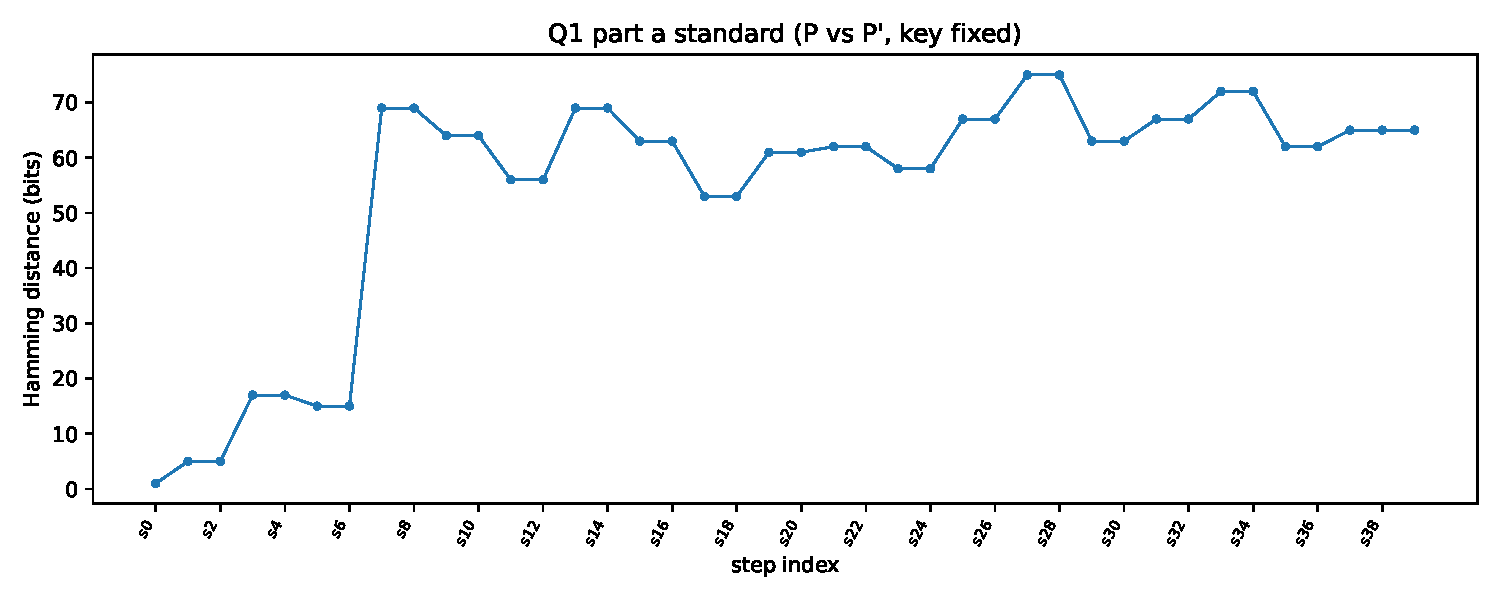
\includegraphics[width=\linewidth]{q1-hamming-rounds.pdf}
\caption{Hamming distance (bits) after each traced AES step: baseline (Part~A).}
\label{fig:q1-hamming-rounds}
\end{figure}
\begin{figure}[htbp]
\centering
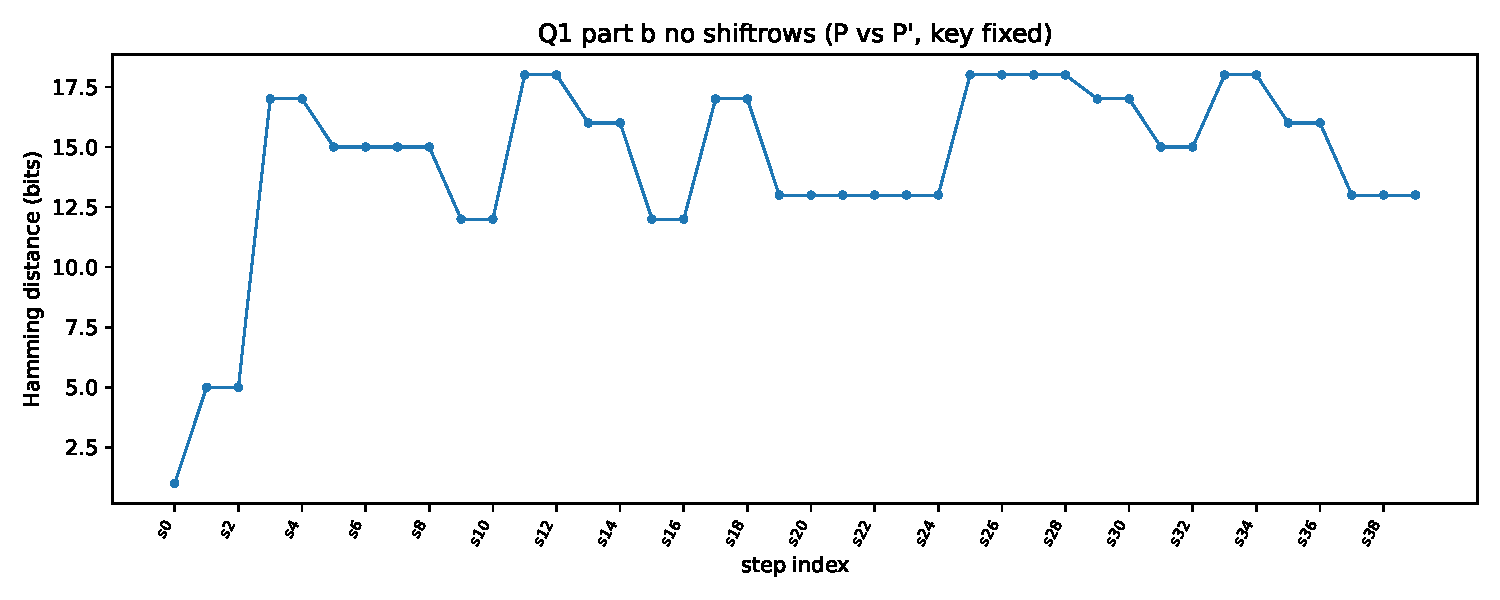
\includegraphics[width=\linewidth]{q1-ablation-shiftrows.pdf}
\caption{Same metric with ShiftRows disabled (Part~B ablation).}
\label{fig:q1-ablation-shiftrows}
\end{figure}
\begin{figure}[htbp]
\centering
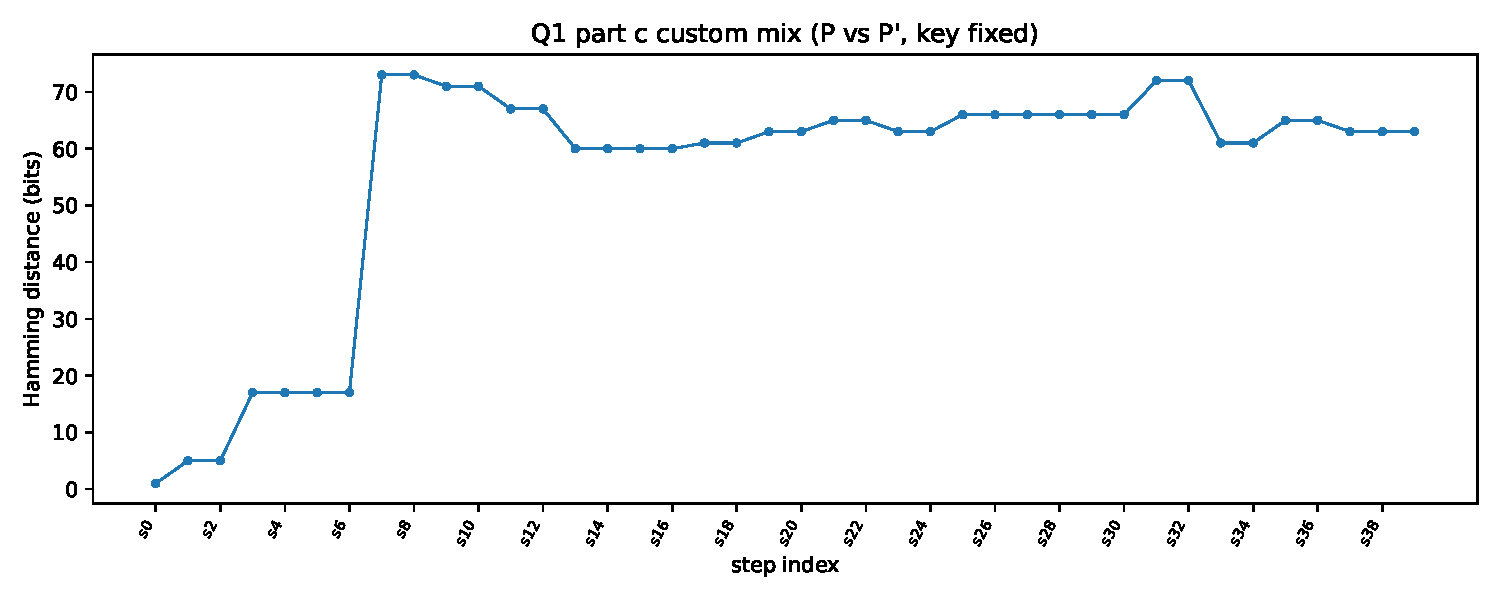
\includegraphics[width=\linewidth]{q1-ablation-mixcolumns.pdf}
\caption{Same metric with custom MixColumns matrix (Part~C ablation).}
\label{fig:q1-ablation-mixcolumns}
\end{figure}

\subsection{Question 2: ECB versus CBC on bitmap data}
OpenSSL encrypts \texttt{assets/Secret.bmp} under AES-128-ECB and AES-128-CBC (PKCS\#7 padding, \texttt{-nosalt}). Figure~\ref{fig:q2-ecb-cbc-noise} visualizes ciphertext byte bodies; Figure~\ref{fig:q2-header-fixed} prepends the plaintext BMP header to ciphertext for quick visual comparison (coursework-style header fix).
\begin{figure}[htbp]
\centering
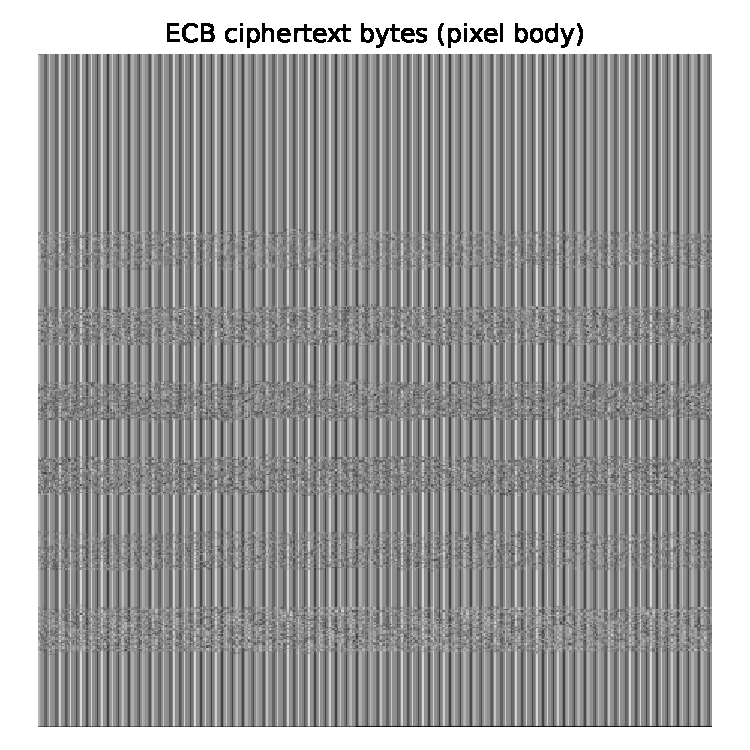
\includegraphics[width=0.42\linewidth]{q2-ecb-noise.pdf}\hfill
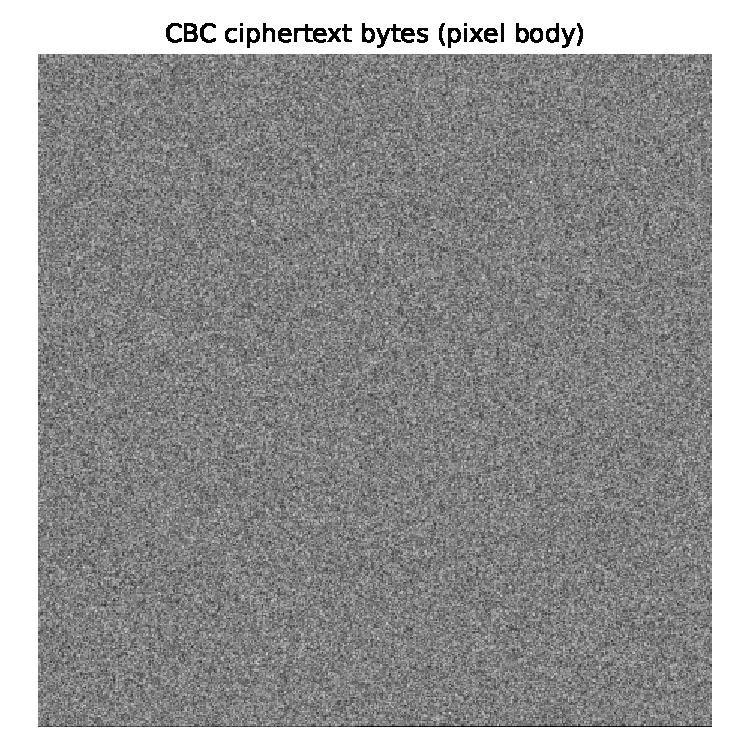
\includegraphics[width=0.42\linewidth]{q2-cbc-noise.pdf}
\caption{Ciphertext-body previews: ECB (left) and CBC (right).}
\label{fig:q2-ecb-cbc-noise}
\end{figure}
\begin{figure}[htbp]
\centering
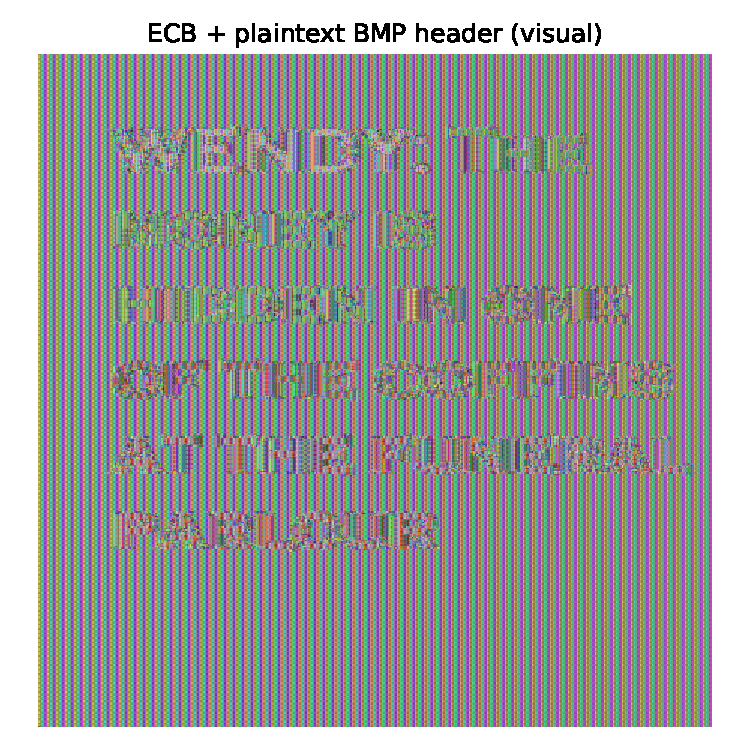
\includegraphics[width=0.42\linewidth]{q2-header-fixed-ecb.pdf}\hfill
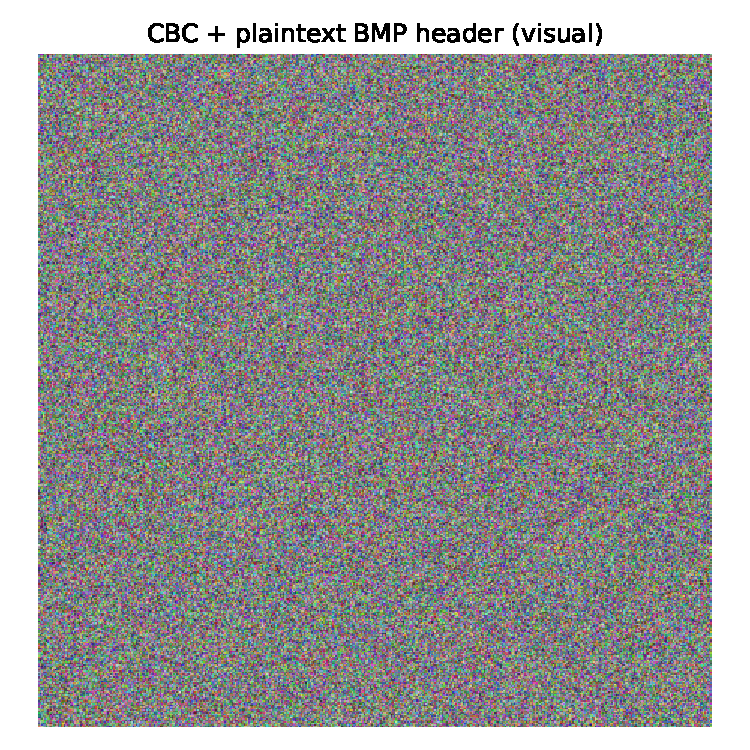
\includegraphics[width=0.42\linewidth]{q2-header-fixed-cbc.pdf}
\caption{Plaintext BMP header applied to ECB (left) and CBC (right) ciphertext.}
\label{fig:q2-header-fixed}
\end{figure}

\subsection{Question 3: TLS negotiation snapshot}
OpenSSL \texttt{s\_client} captures negotiated protocol and cipher for nine public hosts; Figures~\ref{fig:q3-client-hello-table} and~\ref{fig:q3-server-hello-summary} summarize the sample. Full Wireshark ClientHello inventories for two browsers remain in \texttt{output/diagrams/q3-wireshark/}.
\begin{figure}[htbp]
\centering
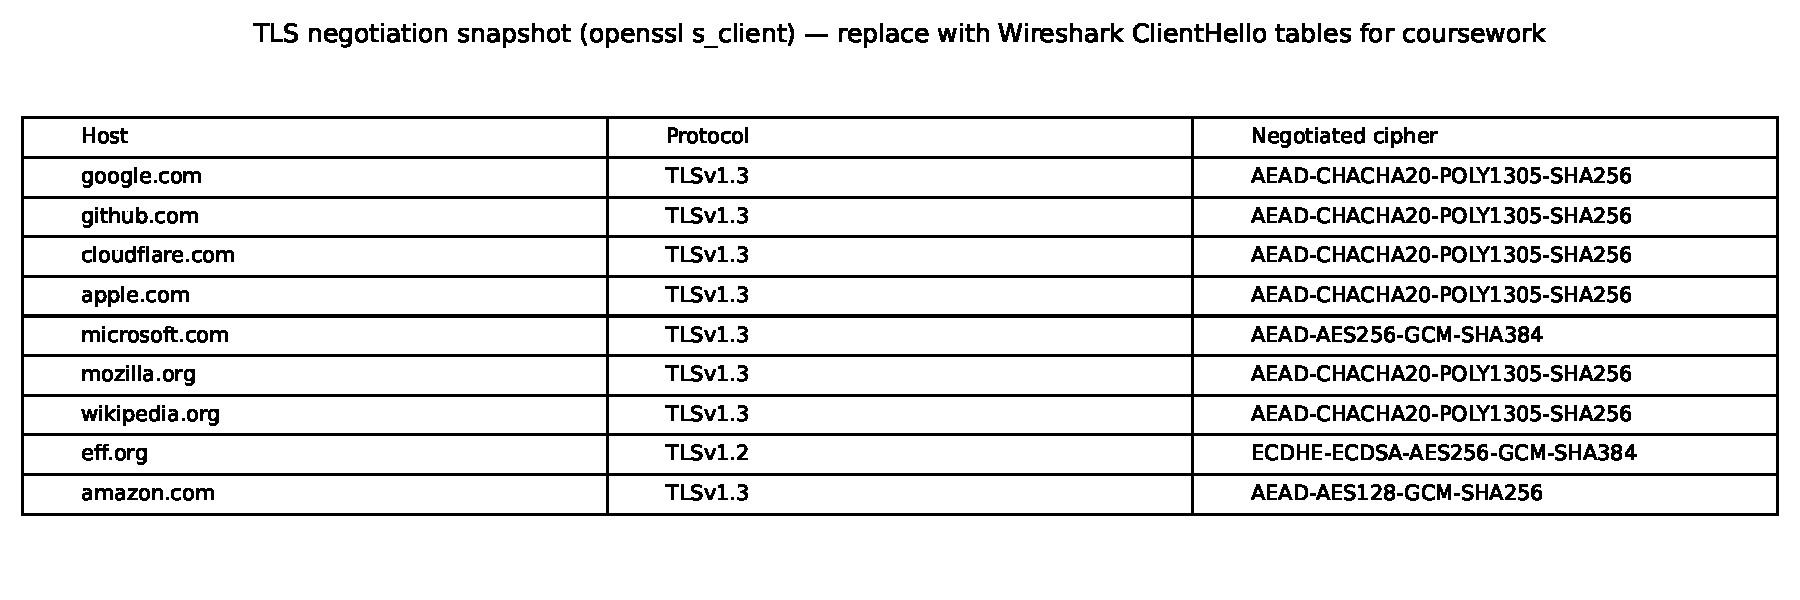
\includegraphics[width=\linewidth]{q3-client-hello-table.pdf}
\caption{Negotiated TLS parameters (openssl-derived stand-in for suite-offer tables).}
\label{fig:q3-client-hello-table}
\end{figure}
\begin{figure}[htbp]
\centering
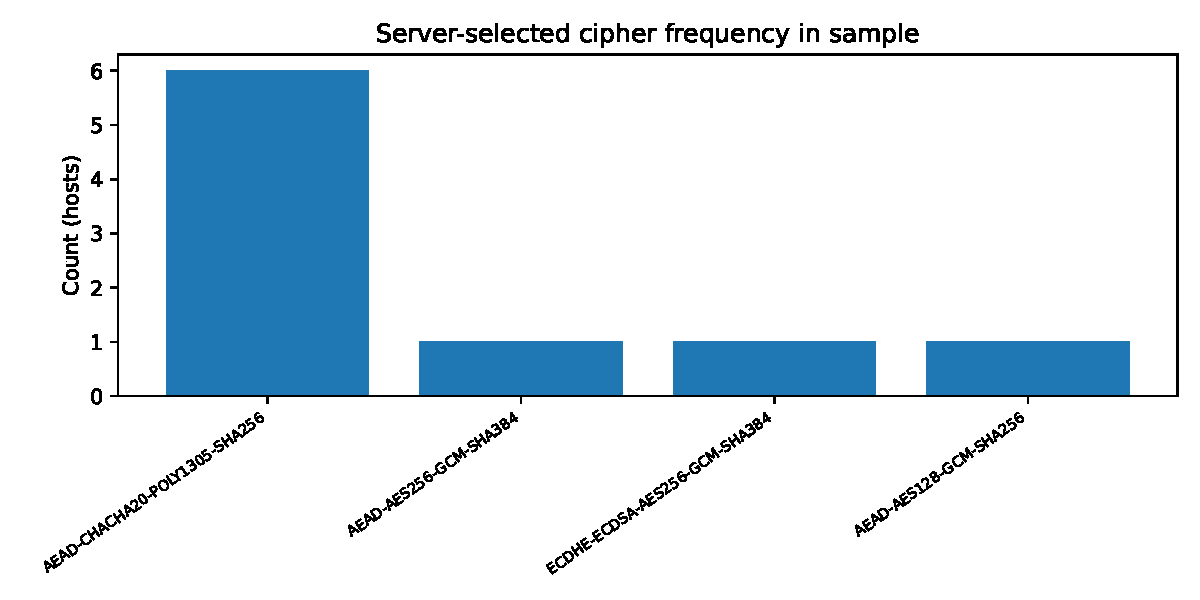
\includegraphics[width=0.85\linewidth]{q3-server-hello-summary.pdf}
\caption{Frequency of server-selected ciphers in the nine-host sample.}
\label{fig:q3-server-hello-summary}
\end{figure}

\subsection{Template demo diagrams (\texttt{examples/python})}
Plots \texttt{performance.pdf} / \texttt{performance.png} under \texttt{output/diagrams/} come from \texttt{examples/python/generate\_results.py} and \texttt{plot\_diagram.py} (not \texttt{run\_coursework\_outputs.py}). Include \texttt{performance.pdf} in the article when every diagram in that directory should appear.
\begin{figure}[htbp]
\centering
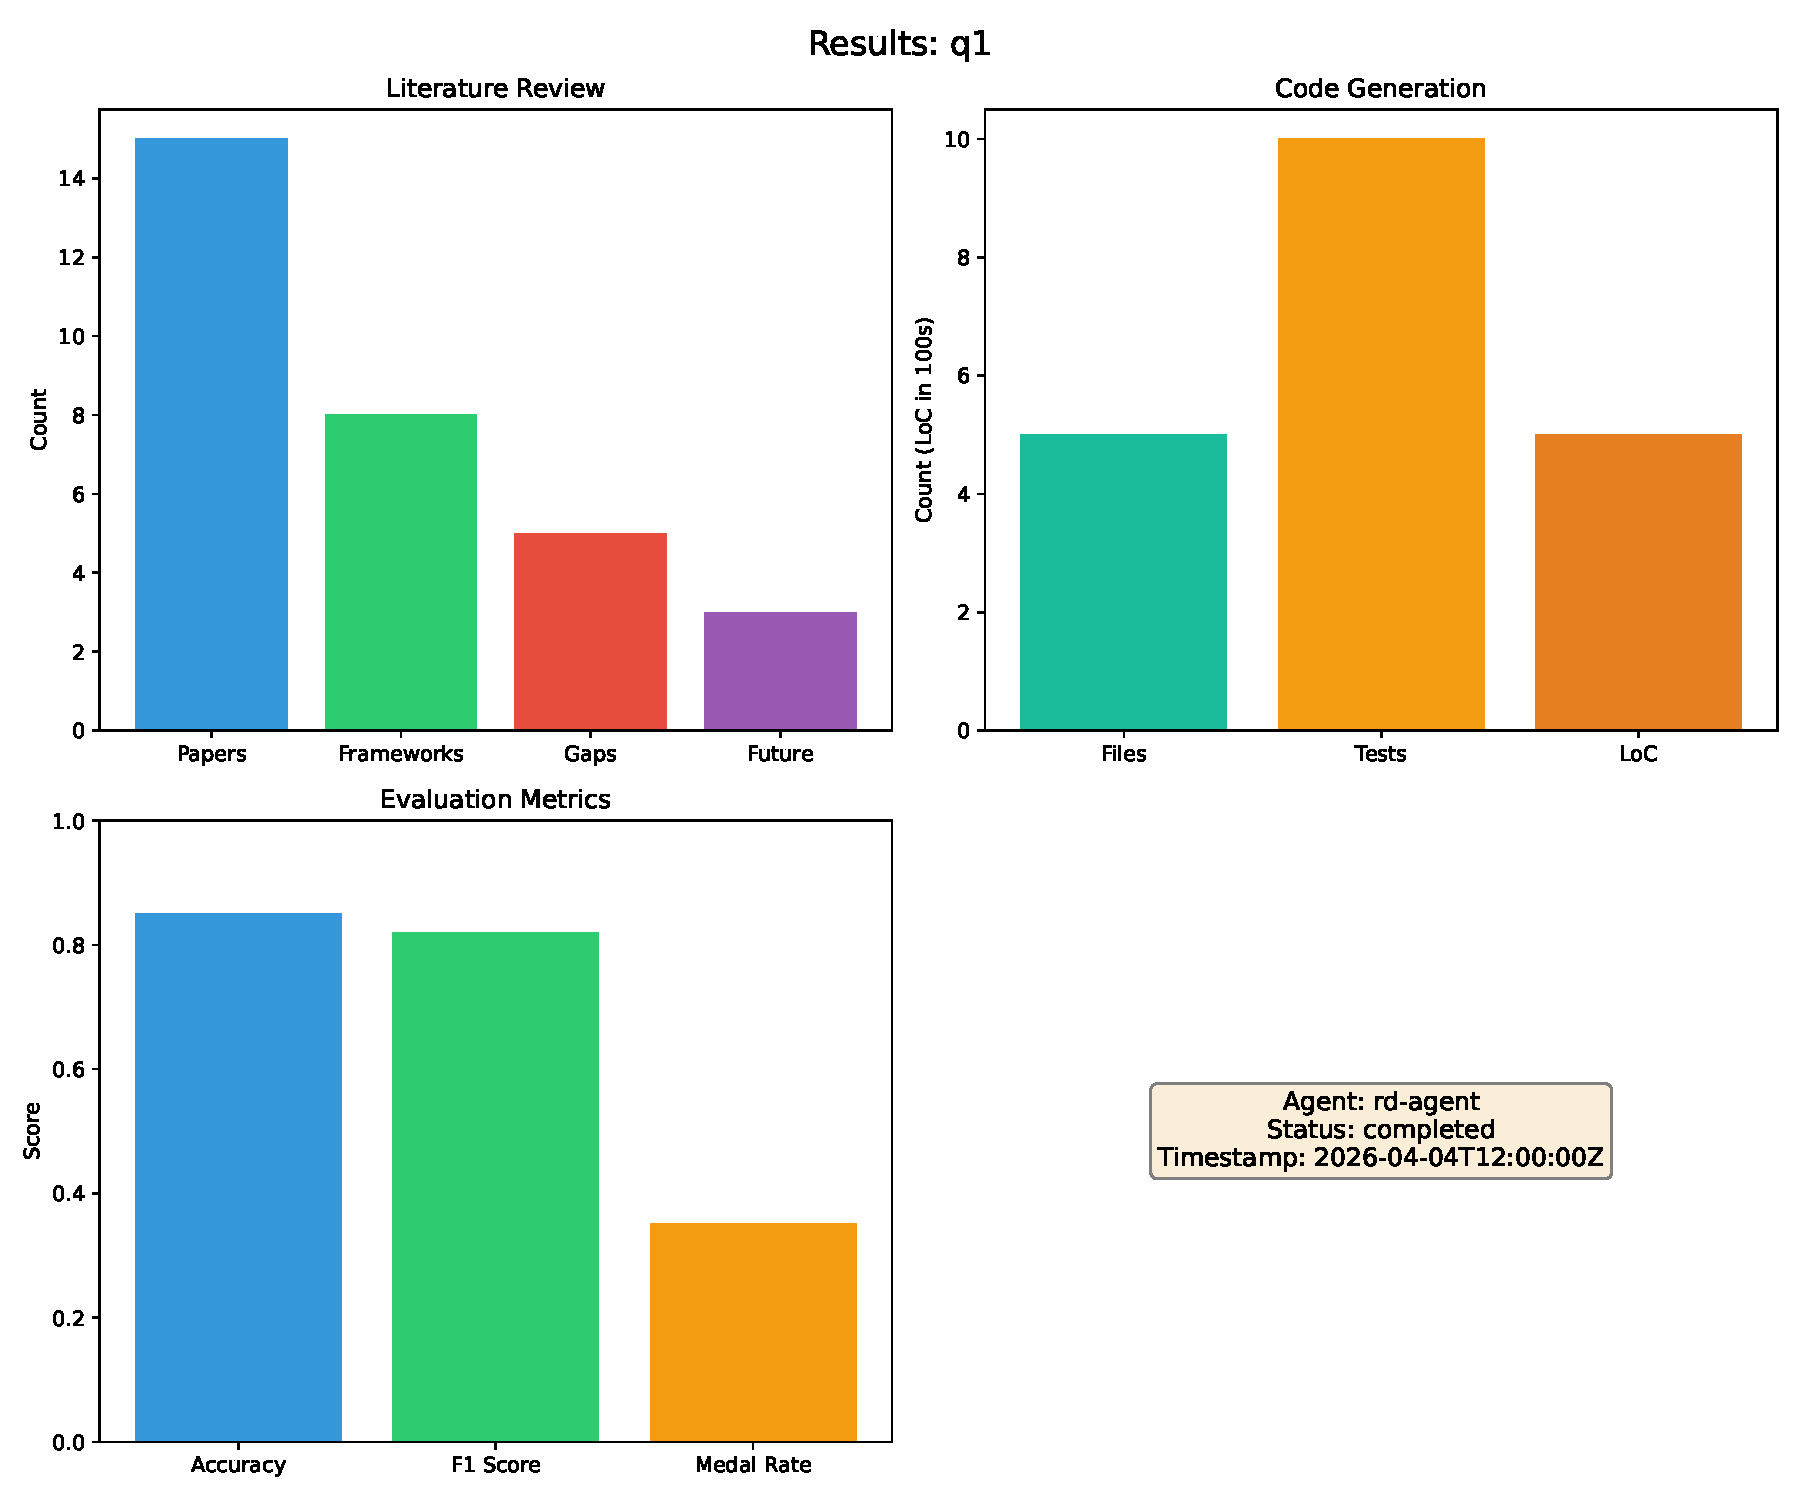
\includegraphics[width=\linewidth]{performance.pdf}
\caption{Demo pipeline metrics (synthetic); from \texttt{plot\_diagram.py}.}
\label{fig:performance-demo}
\end{figure}

% Section 4 | Literature Review \& Positioning | All Members
\section{Literature Review and Positioning}
\label{sec:literature-review}

NIST standardization of AES and guidance on modes and TLS protocol evolution provide the backdrop for our experiments. We cite standard references and optional survey material generated by the research pipeline.

\strength{Positioning against Daemen--Rijmen~\cite{daemen2002design} anchors the AES discussion in the canonical design reference rather than informal summaries.}

\weakness{The bibliography is minimal; TLS ecosystem references (RFCs, surveys) are not yet expanded here.}

\suggestion{Add citations for TLS~1.3 (e.g., RFC~8446) and for classic ECB/CBC misuse examples to strengthen positioning for non-specialist readers.}

% Section 5 | Presentation \& Clarity | Scott Weeden
\section{Presentation and Clarity}
\label{sec:presentation-clarity}

Figures are organized by assignment question with consistent naming (\texttt{q1-}, \texttt{q2-}, \texttt{q3-}) and paths documented in the repository. JSON summaries under \texttt{output/results/} complement the PDF plots for machine-readable replay.

\strength{The ECB/CBC side-by-side layout makes mode leakage visually immediate for instructional use.}

\suggestion{Consider a single roadmap figure or table listing question ID, primary artifact path, and the section where it is interpreted.}

% Section 6 | Detailed Technical Comments | All Members
\section{Detailed Technical Comments}
\label{sec:detailed-comments}

Courseware-scale samples are not representative of global TLS deployment; AES tracing code is for education, not production side-channel resistance. Header repair on ciphertext for BMP viewing is a teaching device and must not be read as a security mechanism.

\weakness{OpenSSL \texttt{s\_client} summaries substitute for full Wireshark ClientHello inventories in part of the TLS discussion; readers should treat the nine-host table as illustrative.}

\suggestion{Where MixColumns is replaced by \texttt{M\_new}, paste or cite the exact matrix from the assignment brief in an appendix to remove ambiguity across course editions.}

% Section 7 | Questions for Authors | All Members
\section{Questions for Authors}
\label{sec:questions-authors}

\begin{itemize}
  \item Can the diffusion plots be extended to multiple random plaintext pairs (e.g., ten variants) with aggregate statistics, as suggested in typical avalanche coursework prompts?
  \item Should TLS results be harmonized strictly from Wireshark (ClientHello lists) versus OpenSSL negotiated ciphers, and how will version skew between tools be documented?
  \item Is there a plan to publish deterministic seeds or pinned OpenSSL/Wireshark versions in a lockfile or container image for long-term reproducibility?
\end{itemize}

% Section 8 | Minor Issues | Scott Weeden
\section{Minor Issues}
\label{sec:minor-issues}

\begin{itemize}
  \item Ensure \texttt{assets/Secret.bmp} is present or documented when cloning; builds fail silently on missing graphics if paths are wrong.
  \item Verify \texttt{\textbackslash graphicspath} when compiling from a directory other than \texttt{src/} (CI may use a different working directory).
  \item Run spell-check on ``Rijndael,'' ``MixColumns,'' and TLS acronym expansion on first use in each major section if the venue requires it.
\end{itemize}

% Section 9 | Meta-Review \& Integration | Phaninder Reddy Masapeta (Lead)
\section{Meta-Review and Integration}
\label{sec:meta-review}

The three tracks (AES instrumentation, modes on structured data, TLS sampling) form a coherent applied-cryptography lab narrative. Together they reinforce standard lessons: rapid diffusion inside AES rounds, structural failure of ECB on repetitive plaintexts, and the diversity of negotiated TLS stacks in the wild.

\strength{Reproducibility is foregrounded: scripts, output paths, and environment assumptions are stated explicitly.}

\section{Reproducibility}
\label{sec:reproducibility}
Regenerate metrics, JSON summaries, and PDF figures with:
\texttt{conda activate rd-ralph-template \&\& python scripts/run\_coursework\_outputs.py} from the repository root (requires OpenSSL and network access for TLS probes). Outputs land in \texttt{output/results/} and \texttt{output/diagrams/} as referenced by \texttt{test\_cases/rd\_agent/}. Key/IV material for Q2 is recorded under \texttt{output/results/q2/openssl\_run.json} for local replay.

For the LangGraph/MCP pipeline, set \texttt{LM\_STUDIO\_BASE\_URL} and enable \texttt{RD\_AGENT\_MCP\_EXEC\_AGENTS=true} only in trusted environments when spawning real \texttt{rd-agent} / \texttt{adk-ralph} subprocesses from \texttt{rd-agent-mcp}.


\bibliographystyle{IEEEtran}
\begin{thebibliography}{1}
\bibitem{daemen2002design}
J.~Daemen and V.~Rijmen, \textit{The Design of Rijndael: AES---The Advanced Encryption Standard}. Berlin: Springer, 2002.
\end{thebibliography}

\end{document}
